\documentclass[10pt]{beamer}

\usetheme[progressbar=frametitle]{metropolis}
\usepackage{appendixnumberbeamer}

\usepackage{booktabs}

%For linking email and website
\usepackage{hyperref}

%For enumeration as words
\usepackage{blindtext}
\usepackage{enumitem}

\usepackage{xspace}
\newcommand{\themename}{\textbf{\textsc{metropolis}}\xspace}

\newcommand{\codeB}[1]{\texttt{#1}}


\title{Theory of Computation}
\subtitle{Tutorial 5 - NFAs}
\date{}
\author{Cesare Spinoso-Di Piano}

\begin{document}

\maketitle

\begin{frame}{Plan for today}
    \setbeamertemplate{section in toc}[sections numbered]
    \tableofcontents[hideallsubsections]
\end{frame}


\section{NFAs}

\begin{frame}[t]{Introduction to NFAs}
    \textbf{Definition.} A \textbf{\underline{nondeterministic} finite automaton (NFA)} $M$ is a 5 element tuple $M = (Q, \Sigma, \delta, q_0, F)$ where
    \begin{itemize}
        \item $Q$ is the set of all states
        \item $\Sigma$ is the alphabet
        \item \textcolor{red}{*} $\delta$ is the transition function $\delta: Q \times \{\Sigma \cup \{\lambda\} \} \rightarrow 2^Q$
        \item $q_0$ is the (\underline{unique}) initial state
        \item $F$ is the set of final states
    \end{itemize}
    A NFA is a machine that reads an input string and decides whether to accept it.\\
    \textcolor{red}{*\textbf{Unlike a DFA: }}
    The transition function of an NFA can accept $\lambda$ and \textbf{always} returns a set.
\end{frame}


\begin{frame}{Introduction to NFAs}

    \textbf{Consider a NFA M}\\
    Given a string $w$, \textbf{M} tries all possible walks. If, at the end of the string, ANY of the walks end in a final state the string is accepted. Otherwise, it is rejected.\\\bigskip

    \textbf{Definition.} The language \textbf{L(M)} includes all strings (over the alphabet $\Sigma$) that are accepted by \textbf{M}.\\
    {$L(M)$} = \{strings that drive \textbf{M} to a final state\}\\\bigskip
    Formally:\\
    $L(M) = \{w\in \Sigma ^*: \delta ^*(q_0,w) \text{ contains at least one final state}\}$, where $\delta ^*$ is the extended transition function $\delta ^*: Q\times \Sigma ^*\rightarrow 2^Q$.
\end{frame}


\begin{frame}{Example}
    \textbf{Example.} The following is an NFA \textbf{M} where $\textbf{L(M)} = \{a\} \cup \{a^{2k}: k > 0\}$ ($\Sigma \{a\}$).

    \begin{center}
        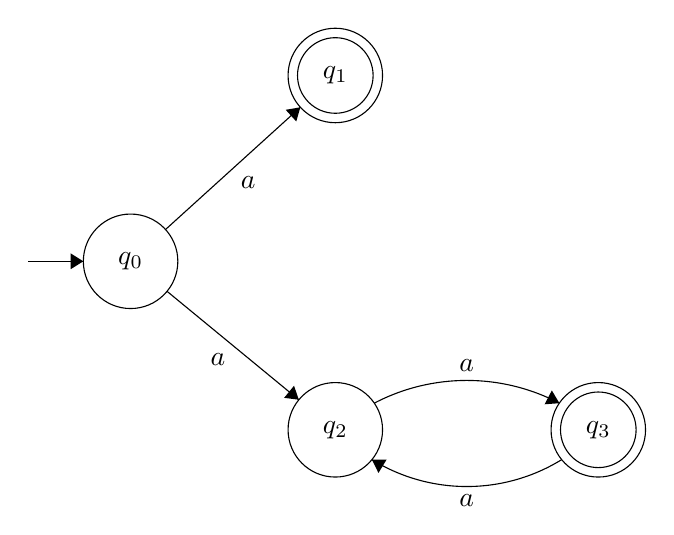
\begin{tikzpicture}[scale=0.2]
            \tikzstyle{every node}+=[inner sep=0pt]
            \draw [black] (8.9,-29.1) circle (3);
            \draw (8.9,-29.1) node {$q_0$};
            \draw [black] (21.9,-17.3) circle (3);
            \draw (21.9,-17.3) node {$q_1$};
            \draw [black] (21.9,-17.3) circle (2.4);
            \draw [black] (21.9,-39.8) circle (3);
            \draw (21.9,-39.8) node {$q_2$};
            \draw [black] (38.6,-39.8) circle (3);
            \draw (38.6,-39.8) node {$q_3$};
            \draw [black] (38.6,-39.8) circle (2.4);
            \draw [black] (2.4,-29.1) -- (5.9,-29.1);
            \fill [black] (5.9,-29.1) -- (5.1,-28.6) -- (5.1,-29.6);
            \draw [black] (11.12,-27.08) -- (19.68,-19.32);
            \fill [black] (19.68,-19.32) -- (18.75,-19.48) -- (19.42,-20.22);
            \draw (16.36,-23.69) node [below] {$a$};
            \draw [black] (11.22,-31.01) -- (19.58,-37.89);
            \fill [black] (19.58,-37.89) -- (19.28,-37) -- (18.65,-37.77);
            \draw (14.45,-34.94) node [below] {$a$};
            \draw [black] (24.37,-38.109) arc (117.6149:62.3851:12.686);
            \fill [black] (36.13,-38.11) -- (35.65,-37.3) -- (35.19,-38.18);
            \draw (30.25,-36.16) node [above] {$a$};
            \draw [black] (36.281,-41.69) arc (-58.29883:-121.70117:11.478);
            \fill [black] (24.22,-41.69) -- (24.64,-42.54) -- (25.16,-41.69);
            \draw (30.25,-43.9) node [below] {$a$};
        \end{tikzpicture}
    \end{center}

\end{frame}

\begin{frame}{Example - Tracing Input}
    $\textbf{L(M)} = \{a\} \cup \{a^{2k}: k > 0\}$\\
    \textbf{Input String: \textcolor{red}{\^{}}aa}

    \begin{center}
        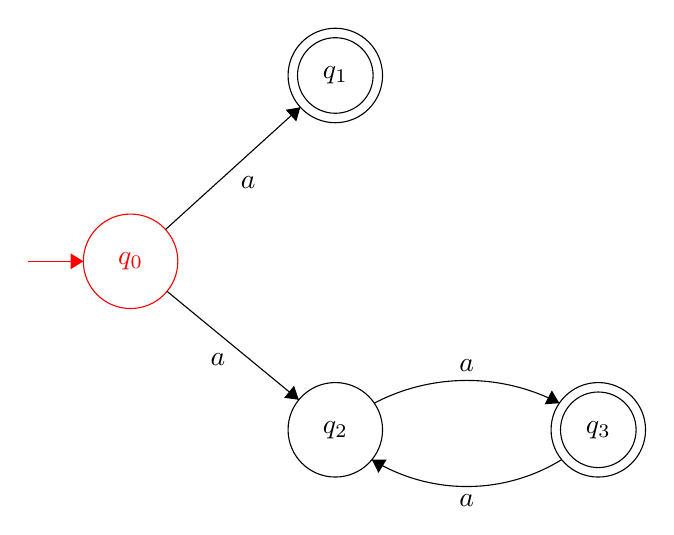
\begin{tikzpicture}[scale=0.2]
            \tikzstyle{every node}+=[inner sep=0pt]
            \draw [red] (8.9,-29.1) circle (3);
            \draw [red] (8.9,-29.1) node {$q_0$};
            \draw [red] [black] (21.9,-17.3) circle (3);
            \draw (21.9,-17.3) node {$q_1$};
            \draw [black] (21.9,-17.3) circle (2.4);
            \draw [black] (21.9,-39.8) circle (3);
            \draw (21.9,-39.8) node {$q_2$};
            \draw [black] (38.6,-39.8) circle (3);
            \draw (38.6,-39.8) node {$q_3$};
            \draw [black] (38.6,-39.8) circle (2.4);
            \draw [red] (2.4,-29.1) -- (5.9,-29.1);
            \fill [red] (5.9,-29.1) -- (5.1,-28.6) -- (5.1,-29.6);
            \draw [black] (11.12,-27.08) -- (19.68,-19.32);
            \fill [black] (19.68,-19.32) -- (18.75,-19.48) -- (19.42,-20.22);
            \draw (16.36,-23.69) node [below] {$a$};
            \draw [black] (11.22,-31.01) -- (19.58,-37.89);
            \fill [black] (19.58,-37.89) -- (19.28,-37) -- (18.65,-37.77);
            \draw (14.45,-34.94) node [below] {$a$};
            \draw [black] (24.37,-38.109) arc (117.6149:62.3851:12.686);
            \fill [black] (36.13,-38.11) -- (35.65,-37.3) -- (35.19,-38.18);
            \draw (30.25,-36.16) node [above] {$a$};
            \draw [black] (36.281,-41.69) arc (-58.29883:-121.70117:11.478);
            \fill [black] (24.22,-41.69) -- (24.64,-42.54) -- (25.16,-41.69);
            \draw (30.25,-43.9) node [below] {$a$};
        \end{tikzpicture}
    \end{center}

\end{frame}

\begin{frame}{Example - Tracing Input}
    $\textbf{L(M)} = \{a\} \cup \{a^{2k}: k > 0\}$\\
    \textbf{Input String: \textcolor{red}aa}

    \begin{center}
        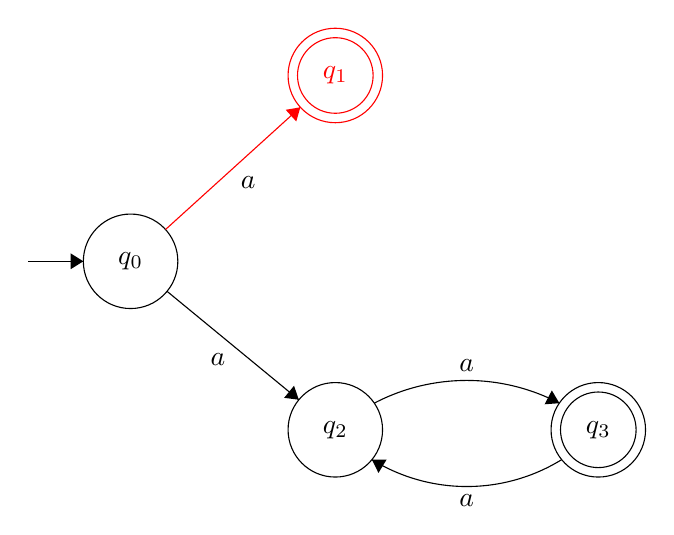
\begin{tikzpicture}[scale=0.2]
            \tikzstyle{every node}+=[inner sep=0pt]
            \draw [black] (8.9,-29.1) circle (3);
            \draw [black] (8.9,-29.1) node {$q_0$};
            \draw [red] (21.9,-17.3) circle (3);
            \draw [red] (21.9,-17.3) node {$q_1$};
            \draw [red] (21.9,-17.3) circle (2.4);
            \draw [black] (21.9,-39.8) circle (3);
            \draw (21.9,-39.8) node {$q_2$};
            \draw [black] (38.6,-39.8) circle (3);
            \draw (38.6,-39.8) node {$q_3$};
            \draw [black] (38.6,-39.8) circle (2.4);
            \draw [black] (2.4,-29.1) -- (5.9,-29.1);
            \fill [black] (5.9,-29.1) -- (5.1,-28.6) -- (5.1,-29.6);
            \draw [red] (11.12,-27.08) -- (19.68,-19.32);
            \fill [red] (19.68,-19.32) -- (18.75,-19.48) -- (19.42,-20.22);
            \draw (16.36,-23.69) node [below] {$a$};
            \draw [black] (11.22,-31.01) -- (19.58,-37.89);
            \fill [black] (19.58,-37.89) -- (19.28,-37) -- (18.65,-37.77);
            \draw (14.45,-34.94) node [below] {$a$};
            \draw [black] (24.37,-38.109) arc (117.6149:62.3851:12.686);
            \fill [black] (36.13,-38.11) -- (35.65,-37.3) -- (35.19,-38.18);
            \draw (30.25,-36.16) node [above] {$a$};
            \draw [black] (36.281,-41.69) arc (-58.29883:-121.70117:11.478);
            \fill [black] (24.22,-41.69) -- (24.64,-42.54) -- (25.16,-41.69);
            \draw (30.25,-43.9) node [below] {$a$};
        \end{tikzpicture}
    \end{center}

\end{frame}

\begin{frame}{Example - Tracing Input}
    $\textbf{L(M)} = \{a\} \cup \{a^{2k}: k > 0\}$\\
    \textbf{Input String: a\textcolor{red}a} \\
    $\delta(q_1, a) = \emptyset$, no where to go. Are we done?

    \begin{center}
        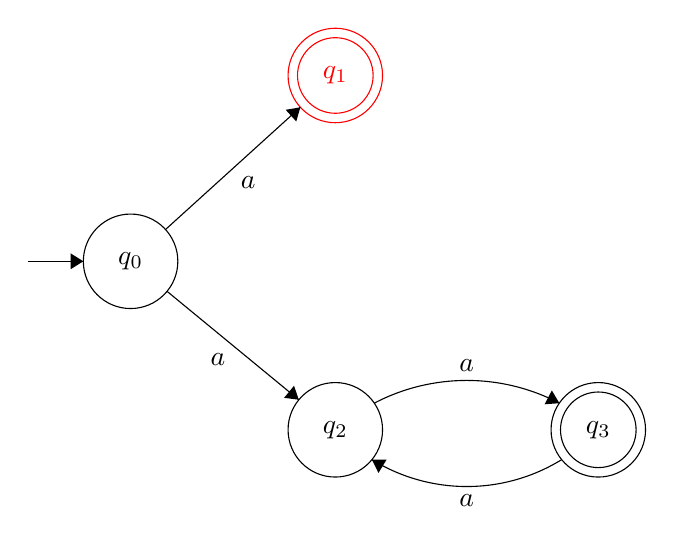
\begin{tikzpicture}[scale=0.2]
            \tikzstyle{every node}+=[inner sep=0pt]
            \draw [black] (8.9,-29.1) circle (3);
            \draw [black] (8.9,-29.1) node {$q_0$};
            \draw [red] (21.9,-17.3) circle (3);
            \draw [red] (21.9,-17.3) node {$q_1$};
            \draw [red] (21.9,-17.3) circle (2.4);
            \draw [black] (21.9,-39.8) circle (3);
            \draw (21.9,-39.8) node {$q_2$};
            \draw [black] (38.6,-39.8) circle (3);
            \draw (38.6,-39.8) node {$q_3$};
            \draw [black] (38.6,-39.8) circle (2.4);
            \draw [black] (2.4,-29.1) -- (5.9,-29.1);
            \fill [black] (5.9,-29.1) -- (5.1,-28.6) -- (5.1,-29.6);
            \draw [black] (11.12,-27.08) -- (19.68,-19.32);
            \fill [black] (19.68,-19.32) -- (18.75,-19.48) -- (19.42,-20.22);
            \draw (16.36,-23.69) node [below] {$a$};
            \draw [black] (11.22,-31.01) -- (19.58,-37.89);
            \fill [black] (19.58,-37.89) -- (19.28,-37) -- (18.65,-37.77);
            \draw (14.45,-34.94) node [below] {$a$};
            \draw [black] (24.37,-38.109) arc (117.6149:62.3851:12.686);
            \fill [black] (36.13,-38.11) -- (35.65,-37.3) -- (35.19,-38.18);
            \draw (30.25,-36.16) node [above] {$a$};
            \draw [black] (36.281,-41.69) arc (-58.29883:-121.70117:11.478);
            \fill [black] (24.22,-41.69) -- (24.64,-42.54) -- (25.16,-41.69);
            \draw (30.25,-43.9) node [below] {$a$};
        \end{tikzpicture}
    \end{center}

\end{frame}

\begin{frame}{Example - Tracing Input}
    $\textbf{L(M)} = \{a\} \cup \{a^{2k}: k > 0\}$\\
    \textbf{Input String: \textcolor{red}{\^{}}aa } \\
    Are we done? No, \textbf{M} tries another walk.

    \begin{center}
        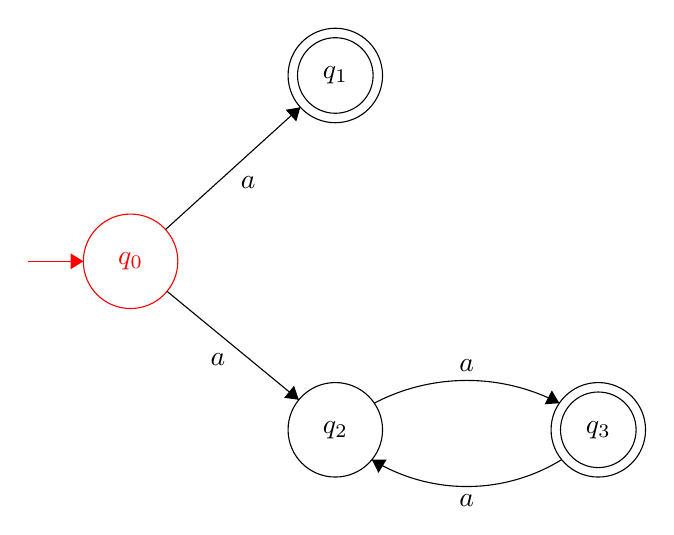
\begin{tikzpicture}[scale=0.2]
            \tikzstyle{every node}+=[inner sep=0pt]
            \draw [red] (8.9,-29.1) circle (3);
            \draw [red] (8.9,-29.1) node {$q_0$};
            \draw [red] [black] (21.9,-17.3) circle (3);
            \draw (21.9,-17.3) node {$q_1$};
            \draw [black] (21.9,-17.3) circle (2.4);
            \draw [black] (21.9,-39.8) circle (3);
            \draw (21.9,-39.8) node {$q_2$};
            \draw [black] (38.6,-39.8) circle (3);
            \draw (38.6,-39.8) node {$q_3$};
            \draw [black] (38.6,-39.8) circle (2.4);
            \draw [red] (2.4,-29.1) -- (5.9,-29.1);
            \fill [red] (5.9,-29.1) -- (5.1,-28.6) -- (5.1,-29.6);
            \draw [black] (11.12,-27.08) -- (19.68,-19.32);
            \fill [black] (19.68,-19.32) -- (18.75,-19.48) -- (19.42,-20.22);
            \draw (16.36,-23.69) node [below] {$a$};
            \draw [black] (11.22,-31.01) -- (19.58,-37.89);
            \fill [black] (19.58,-37.89) -- (19.28,-37) -- (18.65,-37.77);
            \draw (14.45,-34.94) node [below] {$a$};
            \draw [black] (24.37,-38.109) arc (117.6149:62.3851:12.686);
            \fill [black] (36.13,-38.11) -- (35.65,-37.3) -- (35.19,-38.18);
            \draw (30.25,-36.16) node [above] {$a$};
            \draw [black] (36.281,-41.69) arc (-58.29883:-121.70117:11.478);
            \fill [black] (24.22,-41.69) -- (24.64,-42.54) -- (25.16,-41.69);
            \draw (30.25,-43.9) node [below] {$a$};
        \end{tikzpicture}
    \end{center}

\end{frame}

\begin{frame}{Example - Tracing Input}
    $\textbf{L(M)} = \{a\} \cup \{a^{2k}: k > 0\}$\\
    \textbf{Input String: \textcolor{red}aa } \\

    \begin{center}
        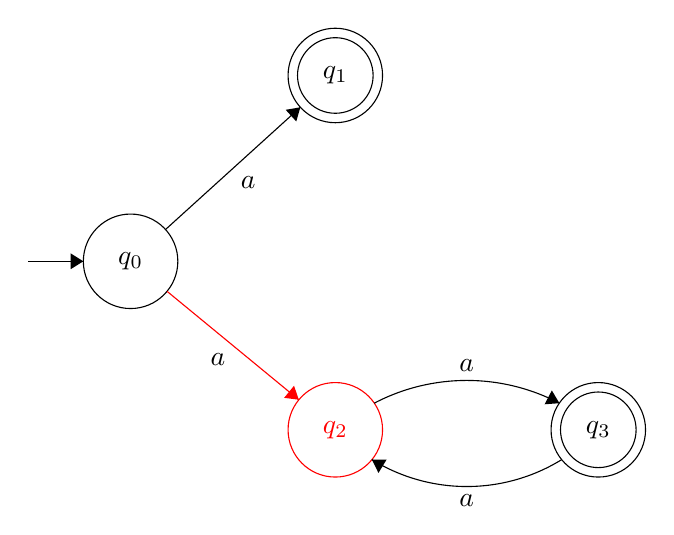
\begin{tikzpicture}[scale=0.2]
            \tikzstyle{every node}+=[inner sep=0pt]
            \draw [black] (8.9,-29.1) circle (3);
            \draw [black] (8.9,-29.1) node {$q_0$};
            \draw [black] (21.9,-17.3) circle (3);
            \draw [black] (21.9,-17.3) node {$q_1$};
            \draw [black] (21.9,-17.3) circle (2.4);
            \draw [red] (21.9,-39.8) circle (3);
            \draw [red] (21.9,-39.8) node {$q_2$};
            \draw [black] (38.6,-39.8) circle (3);
            \draw (38.6,-39.8) node {$q_3$};
            \draw [black] (38.6,-39.8) circle (2.4);
            \draw [black] (2.4,-29.1) -- (5.9,-29.1);
            \fill [black] (5.9,-29.1) -- (5.1,-28.6) -- (5.1,-29.6);
            \draw [black] (11.12,-27.08) -- (19.68,-19.32);
            \fill [black] (19.68,-19.32) -- (18.75,-19.48) -- (19.42,-20.22);
            \draw (16.36,-23.69) node [below] {$a$};
            \draw [red] (11.22,-31.01) -- (19.58,-37.89);
            \fill [red] (19.58,-37.89) -- (19.28,-37) -- (18.65,-37.77);
            \draw (14.45,-34.94) node [below] {$a$};
            \draw [black] (24.37,-38.109) arc (117.6149:62.3851:12.686);
            \fill [black] (36.13,-38.11) -- (35.65,-37.3) -- (35.19,-38.18);
            \draw (30.25,-36.16) node [above] {$a$};
            \draw [black] (36.281,-41.69) arc (-58.29883:-121.70117:11.478);
            \fill [black] (24.22,-41.69) -- (24.64,-42.54) -- (25.16,-41.69);
            \draw (30.25,-43.9) node [below] {$a$};
        \end{tikzpicture}
    \end{center}

\end{frame}



\begin{frame}{Example - Tracing Input}
    $\textbf{L(M)} = \{a\} \cup \{a^{2k}: k > 0\}$\\
    \textbf{Input String: a\textcolor{red}a } \\

    \begin{center}
        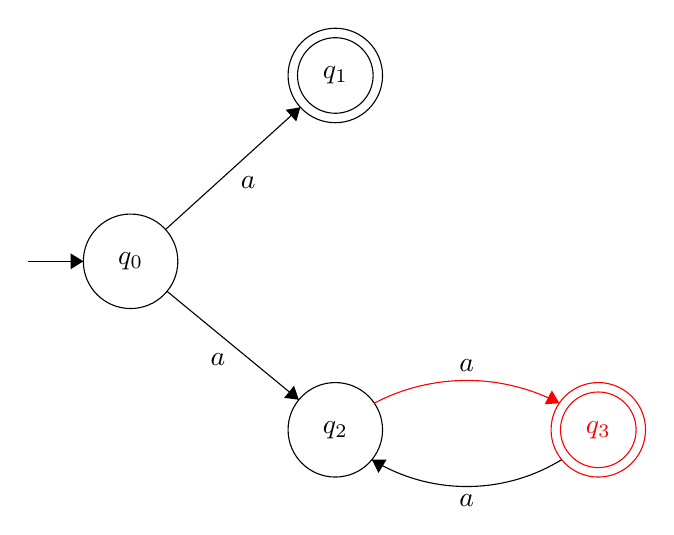
\begin{tikzpicture}[scale=0.2]
            \tikzstyle{every node}+=[inner sep=0pt]
            \draw [black] (8.9,-29.1) circle (3);
            \draw [black] (8.9,-29.1) node {$q_0$};
            \draw [black] (21.9,-17.3) circle (3);
            \draw [black] (21.9,-17.3) node {$q_1$};
            \draw [black] (21.9,-17.3) circle (2.4);
            \draw [black] (21.9,-39.8) circle (3);
            \draw [black] (21.9,-39.8) node {$q_2$};
            \draw [red] (38.6,-39.8) circle (3);
            \draw [red] (38.6,-39.8) node {$q_3$};
            \draw [red] (38.6,-39.8) circle (2.4);
            \draw [black] (2.4,-29.1) -- (5.9,-29.1);
            \fill [black] (5.9,-29.1) -- (5.1,-28.6) -- (5.1,-29.6);
            \draw [black] (11.12,-27.08) -- (19.68,-19.32);
            \fill [black] (19.68,-19.32) -- (18.75,-19.48) -- (19.42,-20.22);
            \draw (16.36,-23.69) node [below] {$a$};
            \draw [black] (11.22,-31.01) -- (19.58,-37.89);
            \fill [black] (19.58,-37.89) -- (19.28,-37) -- (18.65,-37.77);
            \draw (14.45,-34.94) node [below] {$a$};
            \draw [red] (24.37,-38.109) arc (117.6149:62.3851:12.686);
            \fill [red] (36.13,-38.11) -- (35.65,-37.3) -- (35.19,-38.18);
            \draw (30.25,-36.16) node [above] {$a$};
            \draw [black] (36.281,-41.69) arc (-58.29883:-121.70117:11.478);
            \fill [black] (24.22,-41.69) -- (24.64,-42.54) -- (25.16,-41.69);
            \draw (30.25,-43.9) node [below] {$a$};
        \end{tikzpicture}
    \end{center}

    One of the possible walks ends in a final state, \textbf{M} accepts this string.

\end{frame}

\begin{frame}{Example - Tracing Input}
    $\textbf{L(M)} = \{a\} \cup \{a^{2k}: k > 0\}$\\
    \textbf{Input String: aaa} \\

    \begin{center}
        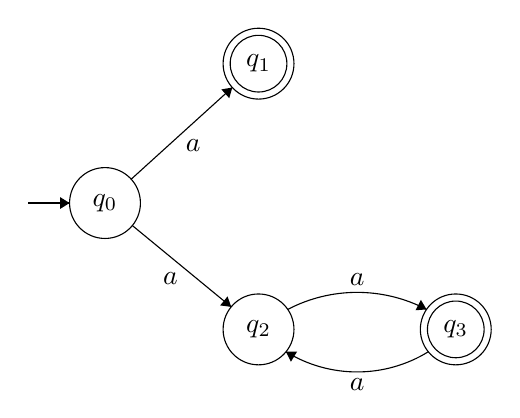
\begin{tikzpicture}[scale=0.15]
            \tikzstyle{every node}+=[inner sep=0pt]
            \draw [black] (8.9,-29.1) circle (3);
            \draw [black] (8.9,-29.1) node {$q_0$};
            \draw [black] (21.9,-17.3) circle (3);
            \draw [black] (21.9,-17.3) node {$q_1$};
            \draw [black] (21.9,-17.3) circle (2.4);
            \draw [black] (21.9,-39.8) circle (3);
            \draw [black] (21.9,-39.8) node {$q_2$};
            \draw [black] (38.6,-39.8) circle (3);
            \draw [black] (38.6,-39.8) node {$q_3$};
            \draw [black] (38.6,-39.8) circle (2.4);
            \draw [black] (2.4,-29.1) -- (5.9,-29.1);
            \fill [black] (5.9,-29.1) -- (5.1,-28.6) -- (5.1,-29.6);
            \draw [black] (11.12,-27.08) -- (19.68,-19.32);
            \fill [black] (19.68,-19.32) -- (18.75,-19.48) -- (19.42,-20.22);
            \draw (16.36,-23.69) node [below] {$a$};
            \draw [black] (11.22,-31.01) -- (19.58,-37.89);
            \fill [black] (19.58,-37.89) -- (19.28,-37) -- (18.65,-37.77);
            \draw (14.45,-34.94) node [below] {$a$};
            \draw [black] (24.37,-38.109) arc (117.6149:62.3851:12.686);
            \fill [black] (36.13,-38.11) -- (35.65,-37.3) -- (35.19,-38.18);
            \draw (30.25,-36.16) node [above] {$a$};
            \draw [black] (36.281,-41.69) arc (-58.29883:-121.70117:11.478);
            \fill [black] (24.22,-41.69) -- (24.64,-42.54) -- (25.16,-41.69);
            \draw (30.25,-43.9) node [below] {$a$};
        \end{tikzpicture}
    \end{center}

    In both traces (top and bottom), do not end up in a final state. \textbf{M} rejects this string.
\end{frame}

\begin{frame}[t]{Exercise}
    \textbf{Exercise.} Given the following NFA \textbf{M},

    \begin{center}
        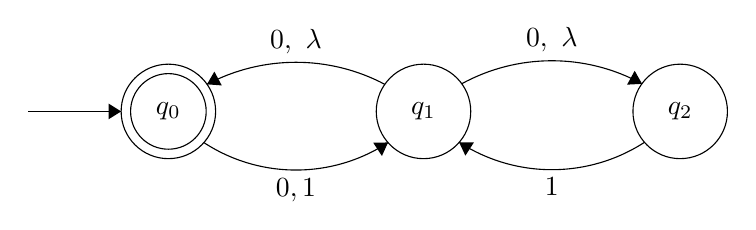
\begin{tikzpicture}[scale=0.2]
            \tikzstyle{every node}+=[inner sep=0pt]
            \draw [black] (13.5,-29.5) circle (3);
            \draw (13.5,-29.5) node {$q_0$};
            \draw [black] (13.5,-29.5) circle (2.4);
            \draw [black] (29.7,-29.5) circle (3);
            \draw (29.7,-29.5) node {$q_1$};
            \draw [black] (46,-29.5) circle (3);
            \draw (46,-29.5) node {$q_2$};
            \draw [black] (4.6,-29.5) -- (10.5,-29.5);
            \fill [black] (10.5,-29.5) -- (9.7,-29) -- (9.7,-30);
            \draw [black] (27.454,-31.474) arc (-56.73531:-123.26469:10.673);
            \fill [black] (27.45,-31.47) -- (26.51,-31.49) -- (27.06,-32.33);
            \draw (21.6,-33.72) node [below] {$0,1$};
            \draw [black] (15.951,-27.783) arc (117.899:62.101:12.074);
            \fill [black] (15.95,-27.78) -- (16.89,-27.85) -- (16.42,-26.97);
            \draw (21.6,-25.88) node [above] {$0,\mbox{ }\lambda$};
            \draw [black] (32.124,-27.746) arc (118.68171:61.31829:11.93);
            \fill [black] (43.58,-27.75) -- (43.11,-26.92) -- (42.63,-27.8);
            \draw (37.85,-25.78) node [above] {$0,\mbox{ }\lambda$};
            \draw [black] (43.74,-31.458) arc (-57.03314:-122.96686:10.824);
            \fill [black] (31.96,-31.46) -- (32.36,-32.31) -- (32.9,-31.47);
            \draw (37.85,-33.7) node [below] {$1$};
        \end{tikzpicture}
    \end{center}

    What is \begin{itemize}
        \item 1. $\delta^*(q_0, 01) = $? Is 01 accepted by this NFA?
    \end{itemize}

\end{frame}

\section{NFA-to-DFA}

\begin{frame}{NFA-to-DFA}
    Given an NFA $N = (Q, \Sigma, \delta, q_0, F)$, how can we convert it to a DFA $M = (Q', \Sigma, \delta', q_0', F')$?\\\bigskip
    Converting a NFA to DFA is also called \textbf{Subset Construction}.\par
    \begin{itemize}
        \item 1) Step 1: Start from the initial state S ($S = \{q_0\}$).
        \item 2) Step 2: For each symbol $a \in \Sigma$, find all the states that can be reached from S: $\delta'(S,a) = \underset{p \in S}\bigcup\delta(p,a)$.
        \item 3) Step 3: Repeat Step 2 on every new state that is generated. Repeat until no new states are produced.
        \item 4) Step 4: Draw the DFA with states and edges from Step 3. \\
    \end{itemize}
    The initial state for the DFA will be $\{q_0\}$. The final states of the DFA will be all those states $S$ that contain a final state from $F$. If the original NFA $N$ accepts $\lambda$, make $\{q_0\}$ a final state.
\end{frame}

\begin{frame}{Example}
    \textbf{Example.} Convert the following NFA $M$ to a DFA. $M$ is the NFA accepting all strings (over $\Sigma = \{0,1\}$) that end in 01.
    \begin{center}
        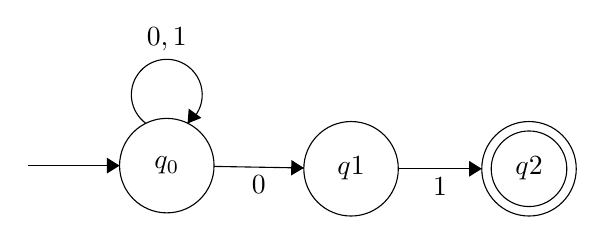
\begin{tikzpicture}[scale=0.2]
            \tikzstyle{every node}+=[inner sep=0pt]
            \draw [black] (19.1,-20.9) circle (3);
            \draw (19.1,-20.9) node {$q_0$};
            \draw [black] (30.8,-21.1) circle (3);
            \draw (30.8,-21.1) node {$q1$};
            \draw [black] (42.1,-21.1) circle (3);
            \draw (42.1,-21.1) node {$q2$};
            \draw [black] (42.1,-21.1) circle (2.4);
            \draw [black] (10.3,-20.9) -- (16.1,-20.9);
            \fill [black] (16.1,-20.9) -- (15.3,-20.4) -- (15.3,-21.4);
            \draw [black] (17.777,-18.22) arc (234:-54:2.25);
            \draw (19.1,-13.65) node [above] {$0,1$};
            \fill [black] (20.42,-18.22) -- (21.3,-17.87) -- (20.49,-17.28);
            \draw [black] (22.1,-20.95) -- (27.8,-21.05);
            \fill [black] (27.8,-21.05) -- (27.01,-20.54) -- (26.99,-21.53);
            \draw (24.94,-21.52) node [below] {$0$};
            \draw [black] (33.8,-21.1) -- (39.1,-21.1);
            \fill [black] (39.1,-21.1) -- (38.3,-20.6) -- (38.3,-21.6);
            \draw (36.45,-21.6) node [below] {$1$};
        \end{tikzpicture}
    \end{center}
\end{frame}

\begin{frame}{Example}
    \textbf{Example.} Converting the NFA $M$ to a DFA:
    \begin{itemize}
        \item 1) Step 1: Start from the start state S. \textcolor{red}{$S=\{q_0\}$}
        \item 2) Step 2: Find all the states that can be reached from S: $\forall a\in\Sigma$, $\delta'(S,a) = \underset{p \in S}\bigcup\delta_{N}(p,a)$.  \textcolor{red}{$\delta'(S,0) = \{q_0, q1\}$, $\delta'(S,1) = \{q_0\}$}
    \end{itemize}
    \begin{center}
        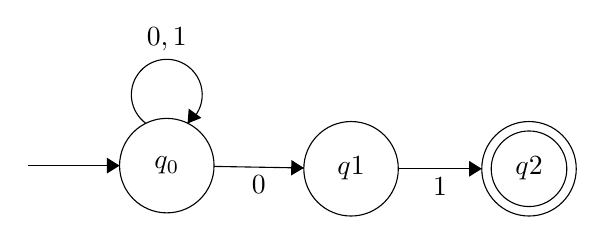
\begin{tikzpicture}[scale=0.2]
            \tikzstyle{every node}+=[inner sep=0pt]
            \draw [black] (19.1,-20.9) circle (3);
            \draw (19.1,-20.9) node {$q_0$};
            \draw [black] (30.8,-21.1) circle (3);
            \draw (30.8,-21.1) node {$q1$};
            \draw [black] (42.1,-21.1) circle (3);
            \draw (42.1,-21.1) node {$q2$};
            \draw [black] (42.1,-21.1) circle (2.4);
            \draw [black] (10.3,-20.9) -- (16.1,-20.9);
            \fill [black] (16.1,-20.9) -- (15.3,-20.4) -- (15.3,-21.4);
            \draw [black] (17.777,-18.22) arc (234:-54:2.25);
            \draw (19.1,-13.65) node [above] {$0,1$};
            \fill [black] (20.42,-18.22) -- (21.3,-17.87) -- (20.49,-17.28);
            \draw [black] (22.1,-20.95) -- (27.8,-21.05);
            \fill [black] (27.8,-21.05) -- (27.01,-20.54) -- (26.99,-21.53);
            \draw (24.94,-21.52) node [below] {$0$};
            \draw [black] (33.8,-21.1) -- (39.1,-21.1);
            \fill [black] (39.1,-21.1) -- (38.3,-20.6) -- (38.3,-21.6);
            \draw (36.45,-21.6) node [below] {$1$};
        \end{tikzpicture}
    \end{center}
\end{frame}

\begin{frame}{Example}
    \textbf{Example.}
    \begin{itemize}
        \item 3) Step 3: Repeat Step 2 on every new state that is generated. Repeat until no new states are produced.

    \end{itemize}
    \begin{center}
        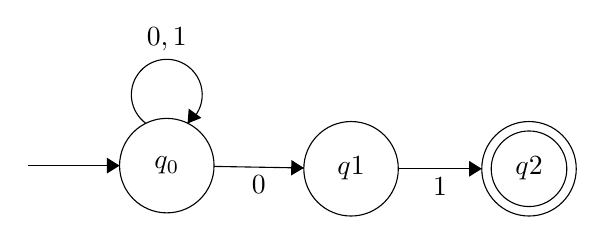
\begin{tikzpicture}[scale=0.2]
            \tikzstyle{every node}+=[inner sep=0pt]
            \draw [black] (19.1,-20.9) circle (3);
            \draw (19.1,-20.9) node {$q_0$};
            \draw [black] (30.8,-21.1) circle (3);
            \draw (30.8,-21.1) node {$q1$};
            \draw [black] (42.1,-21.1) circle (3);
            \draw (42.1,-21.1) node {$q2$};
            \draw [black] (42.1,-21.1) circle (2.4);
            \draw [black] (10.3,-20.9) -- (16.1,-20.9);
            \fill [black] (16.1,-20.9) -- (15.3,-20.4) -- (15.3,-21.4);
            \draw [black] (17.777,-18.22) arc (234:-54:2.25);
            \draw (19.1,-13.65) node [above] {$0,1$};
            \fill [black] (20.42,-18.22) -- (21.3,-17.87) -- (20.49,-17.28);
            \draw [black] (22.1,-20.95) -- (27.8,-21.05);
            \fill [black] (27.8,-21.05) -- (27.01,-20.54) -- (26.99,-21.53);
            \draw (24.94,-21.52) node [below] {$0$};
            \draw [black] (33.8,-21.1) -- (39.1,-21.1);
            \fill [black] (39.1,-21.1) -- (38.3,-20.6) -- (38.3,-21.6);
            \draw (36.45,-21.6) node [below] {$1$};
        \end{tikzpicture}
    \end{center}
    \begin{table}[]
        \begin{tabular}{|r|r|r|ll}
            \cline{1-3}
                                & 0          & 1          &  & \\ \cline{1-3}
            $\rightarrow$\{q0\} & \{q0, q1\} & \{q0\}     &  & \\ \cline{1-3}
            \{q0, q1\}          & \{q0, q1\} & \{q0, q2\} &  & \\ \cline{1-3}
            *\{q0, q2\}         & \{q0, q1\} & \{q0\}     &  & \\ \cline{1-3}
        \end{tabular}
    \end{table}
\end{frame}

\begin{frame}{Example}
    \textbf{Example.}
    \begin{itemize}
        \item 4) Step 4: Draw the DFA

    \end{itemize}
    \begin{table}[]
        \begin{tabular}{|r|r|r|ll}
            \cline{1-3}
                                & 0          & 1          &  & \\ \cline{1-3}
            $\rightarrow$\{q0\} & \{q0, q1\} & \{q0\}     &  & \\ \cline{1-3}
            \{q0, q1\}          & \{q0, q1\} & \{q0, q2\} &  & \\ \cline{1-3}
            *\{q0, q2\}         & \{q0, q1\} & \{q0\}     &  & \\ \cline{1-3}
        \end{tabular}
    \end{table}
    \begin{center}
        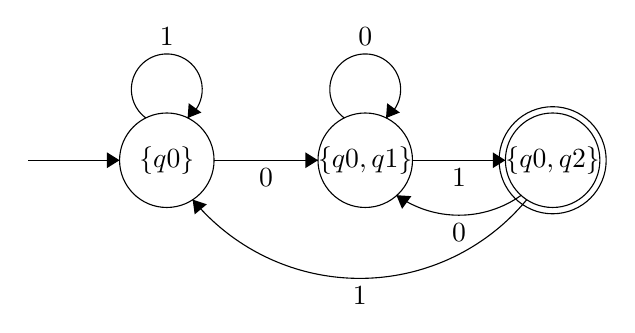
\begin{tikzpicture}[scale=0.2]
            \tikzstyle{every node}+=[inner sep=0pt]
            \draw [black] (18.9,-21.1) circle (3);
            \draw (18.9,-21.1) node {$\{q0\}$};
            \draw [black] (31.5,-21.1) circle (3);
            \draw (31.5,-21.1) node {$\{q0,q1\}$};
            \draw [black] (43.4,-21.1) circle (3.4);
            \draw (43.4,-21.1) node {$\{q0,q2\}$};
            \draw [black] (43.4,-21.1) circle (3);
            \draw [black] (10.1,-21.1) -- (15.9,-21.1);
            \fill [black] (15.9,-21.1) -- (15.1,-20.6) -- (15.1,-21.6);
            \draw [black] (17.577,-18.42) arc (234:-54:2.25);
            \draw (18.9,-13.85) node [above] {$1$};
            \fill [black] (20.22,-18.42) -- (21.1,-18.07) -- (20.29,-17.48);
            \draw [black] (21.9,-21.1) -- (28.5,-21.1);
            \fill [black] (28.5,-21.1) -- (27.7,-20.6) -- (27.7,-21.6);
            \draw (25.2,-21.6) node [below] {$0$};
            \draw [black] (34.5,-21.1) -- (40.4,-21.1);
            \fill [black] (40.4,-21.1) -- (39.6,-20.6) -- (39.6,-21.6);
            \draw (37.45,-21.6) node [below] {$1$};
            \draw [black] (41.416,-23.318) arc (-54.41125:-125.58875:6.816);
            \fill [black] (33.48,-23.32) -- (33.84,-24.19) -- (34.43,-23.38);
            \draw (37.45,-25.09) node [below] {$0$};
            \draw [black] (30.177,-18.42) arc (234:-54:2.25);
            \draw (31.5,-13.85) node [above] {$0$};
            \fill [black] (32.82,-18.42) -- (33.7,-18.07) -- (32.89,-17.48);
            \draw [black] (41.757,-23.603) arc (-39.52969:-140.47031:13.752);
            \fill [black] (20.54,-23.6) -- (20.67,-24.54) -- (21.44,-23.9);
            \draw (31.15,-29.1) node [below] {$1$};
        \end{tikzpicture}
    \end{center}
\end{frame}

\begin{frame}{Theorem}
    \textbf{Theorem. }The set of all languages accepted by NFAs is the same as the set of all languages accepted by DFAs.\\
    Why?
    \begin{itemize}
        \item 1. Every DFA is an NFA.
        \item 2. Every NFA can be converted into a DFA.
    \end{itemize}
    \textbf{Corollary. }A language is regular if there is an FA (either DFA or NFA) that accepts it.
\end{frame}


\end{document}





